\newpage
\section{Fuente de corriente controlada por tensión}
\onehalfspacing
\begin{figure}[htb]
	\centering
	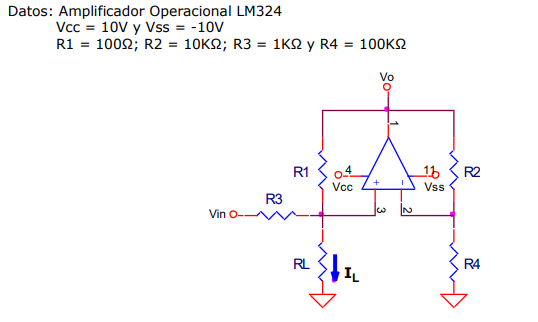
\includegraphics[width=1\textwidth]{figuras/circuito2_consigna.png}
	\caption{Circuito propuesto}
\end{figure}
\subsection{Análisis teórico}
Para analizar el circuito propuesto, se propone expresar $V^+$ (la entrada no inversora del AO) y $V^-$ (la entrada inversora del AO) en función del Vo, planteando el divisor resistivo en el nodo "2" de la figura:
\begin{center}
	$V^+ = V^- = V_o \frac{R_4}{R_4 + R_2}$
\end{center}
luego se plantea la ley de los nodos de Kirchhoff en el nodo "3"
\begin{center}
	$\frac{V_{in} - V^+ }{R_3} + \frac{V_o - V^+ }{R_1} = \frac{V^+}{R_L}$
\end{center}
\begin{center}
	$\frac{V_{in}}{R_3} + \frac{V_o}{R_1} = V^+ (\frac{1}{R_L} + \frac{1}{R_1} + \frac{1}{R_3})$
\end{center}
y reemplazando $V^+$
\begin{center}
	$\frac{V_{in}}{R_3} + \frac{V_o}{R_1} = V_o \frac{R_4}{R_4 + R_2} (\frac{1}{R_L} + \frac{1}{R_1} + \frac{1}{R_3})$
\end{center}
\begin{center}
	$V_{in} = V_o[\frac{1}{R_L}( R_3 \frac{R_4}{R_4 + R_2}) + (R_3 \frac{R_4}{R_4 + R_2}) (\frac{1}{R_1} + \frac{1}{R_3} ) - \frac{R_3}{R_1}]$
\end{center}
Reemplazando para $R_1=100[\Omega]$, $R_2=10[K\Omega]$, $R_3=1[K\Omega]$ y $R_4=100[K\Omega]$:
\begin{center}
	$V_{in} = V_o[\frac{1}{R_L}(909.09091)]$
\end{center}
Luego la corriente que circula por la carga se define:
\begin{center}
	$I_{RL} = \frac{V^+}{R_L}$
\end{center}
\begin{center}
	$I_{RL} = V_o \frac{R_4}{R_4 + R_2} \frac{1}{R_L}$
\end{center}
\begin{center}
	$I_{RL} = \frac{V_{in}}{[\frac{1}{R_L}( R_3 \frac{R_4}{R_4 + R_2}) + (R_3 \frac{R_4}{R_4 + R_2}) (\frac{1}{R_1} + \frac{1}{R_3} ) - \frac{R_3}{R_1}]} \frac{R_4}{R_4 + R_2} \frac{1}{R_L}$
\end{center}
\begin{center}
	$I_{RL} = \frac{V_{in}}{R_3}$
\end{center}
\begin{center}
	\boxed{I_{RL} = V_{in} 10^{-3}} 
\end{center}
de igual manera se define la tensión $V_o$ en función de $R_L$ y de $V_{in}$
\begin{center}
	$V_o = \frac{V_{in}}{(\frac{1}{R_L} (909.09091))}$
\end{center}
\begin{center}
	\boxed{V_o = V_{in} R_L (1.1 *10^{-3})} 
\end{center}
Por último, se determina el valor de $R_{Lmax}$ teniendo en cuenta que al ser ideal el A.O. la tensión de salida máxima será la misma que $V_{cc} = 10[V]$. Por lo tanto operando se obtiene:
\begin{center}
	\boxed{R_{Lmax}= \frac{9090.9091}{V_{in}}} 
\end{center}
A partir de las relaciones obtenidas, se procede a completar la siguiente tabla:
\begin{table}[H]
	\begin{center}
		\begin{tabular}{| c | c | c | c | c |}
			\hline
			\multicolumn{2}{ |c| }{-} &
			\multicolumn{3}{ |c| }{$V_{in}$[V]} \\ \hline
			
			\multicolumn{2}{ |c| }{$I_{RL}$[\textmu A]} & 0.5 & 1 & 2 \\ \hline
			\multirow{5}{*}{$R_L$[K$\Omega$]}	&  0 &   0 &    0  &   0 \\
			&  1 & 500 & 1000 & 2000 \\
			&  2 & 500 & 1000 & 2000 \\
			&  5 & 500 & 1000 & 2000 \\
			& 10 & 500 & 1000 & 2000 \\ \hline
	
		\end{tabular}
				\caption{Valores teóricos de $I_{RL}$ en función de $R_L$ y de $V_{in}$}
		\end{center}
\end{table} 

\begin{table}[H]
	\begin{center}
		\begin{tabular}{| c | c | c | c | c |}
			\hline
			\multicolumn{2}{ |c| }{-} &
			\multicolumn{3}{ |c| }{$V_{in}$[V]} \\ \hline
			
			\multicolumn{2}{ |c| }{$V_o$[V]} & 0.5 & 1 & 2 \\ \hline
			\multirow{5}{*}{$R_L$[K$\Omega$]} & 0	& 0    & 0   & 0   \\
			& 1	& 0.55 & 1.1 & 2.2 \\
			& 2	& 1.1  & 2.2 & 4.4 \\
			& 5	& 2.75 & 5.5 & 11  \\
			& 10	& 5.5  & 11  & 22  \\ \hline
			
		\end{tabular}
		\caption{Valores teóricos de $V_o$ en función de $R_L$ y de $V_{in}$}
	\end{center}
\end{table} 
Aquellos valores que superen el valor de la tensión de $V_{cc}$, la salida se enclava a ese mismo valor y la forma de la onda se recorta.


\subsection{Simulaciones}
Se realizaron diferentes simulaciones con LTSpice para observar el comportamiento de $I_{RL}$ y $V_o$. 
Luego se completaron nuevamente las tablas anteriores con los valores simulados.

\begin{figure}[H]
	\centering
	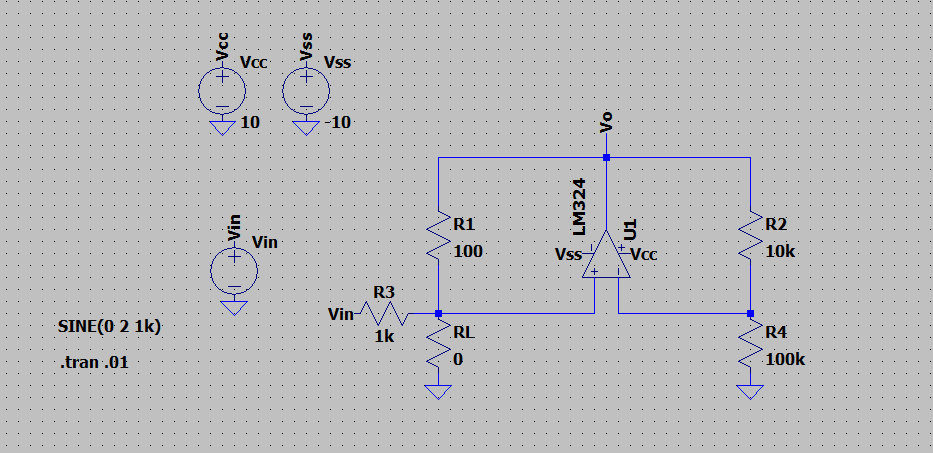
\includegraphics[width=1\textwidth]{figuras/circuito2.png}
	\caption{Circuito simulado}
\end{figure}
\begin{figure}[H]
	\centering
	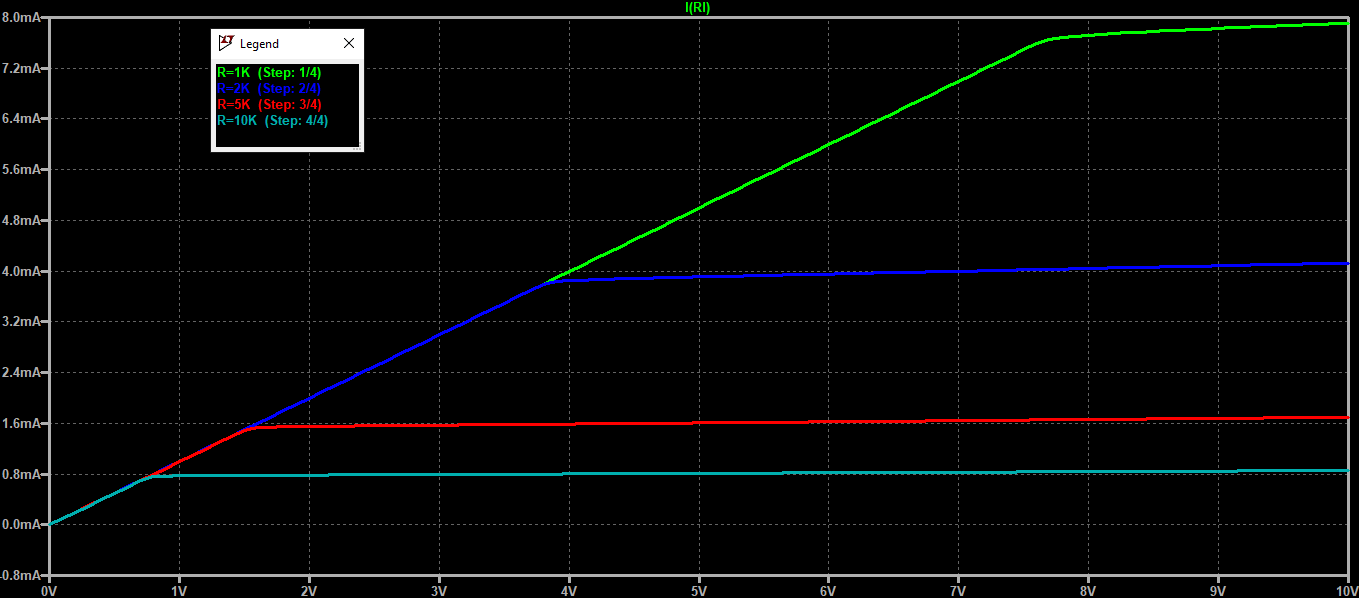
\includegraphics[width=1\textwidth]{figuras/dcsweep_rl.png}
	\caption{$I_{RL} = f(R_L , V_{in})$}
\end{figure}
Para esta simulación se hizo un barrido en continua de 0[V] a 10[V], ya que desde -10[V] la respuesta es aproximadamente simétrica. Lo que se observa es que la variación de la corriente es lineal hasta el punto de tensión para cada valor de $R_L$  que satura al operacional. 
\begin{center}
	\begin{tabular}{| c | c |}
		\hline
		      $R_L$     &   $V_{in-sat}$ \\ \hline
		 1 [K$\Omega$] 	&   	7.5 [V]	 \\
		 2 [K$\Omega$] 	&  	    3.5 [V]	 \\
		 5 [K$\Omega$] 	&    	1.4 [V]	 \\
		10 [K$\Omega$] 	&   	0.5 [V]	 \\ \hline
		
	\end{tabular}
	\begin{figure}[H]
		\centering
		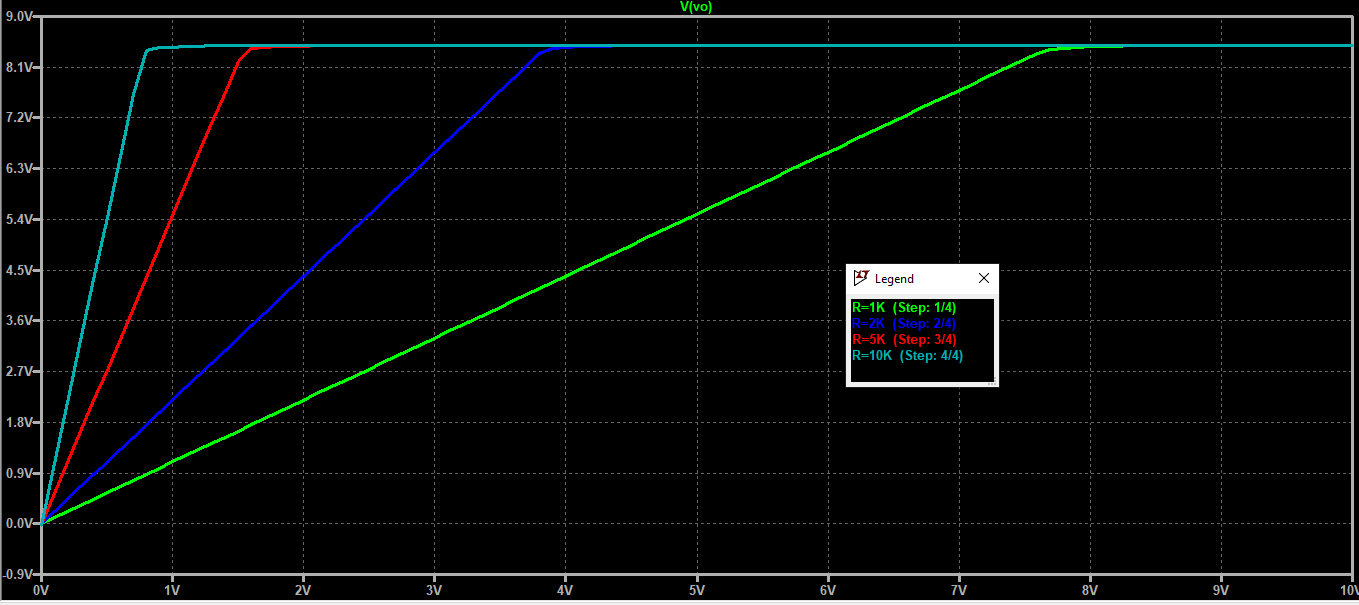
\includegraphics[width=1\textwidth]{figuras/dcsweep_vo.png}
		\caption{$V_o = f(V_{in}, R_L)$}
	\end{figure}
\end{center}
	Aqui se observa como varía la tensión de salida respecto a la tensión de entrada y a los valores de $R_L$ propuestos.
\begin{table}[H]
	\begin{center}
		\begin{tabular}{| c | c | c | c | c |}
			\hline
			\multicolumn{2}{ |c| }{-} &
			\multicolumn{3}{ |c| }{$V_{in}$[V]} \\ \hline
			
			\multicolumn{2}{ |c| }{$I_{RL}$[\textmu A]} 
									 & 0.5    & 1 	   &    2 \\ \hline
			
	\multirow{5}{*}{$R_L$[K$\Omega$]} 	&  0 &   0    &   0    &    0 \\
				&  1 & 495.93 & 994.15 & 1994.08 \\
				&  2 & 495.52 & 993.33 & 1991.35 \\
				&  5 & 493.86 & 990.39 & 1549.12 \\
				& 10 & 488.45 & 771.00 &  783.06 \\ \hline
			
		\end{tabular}
		\caption{Valores simulados de $I_{RL}$ en función de $R_L$ y de $V_{in}$}
	\end{center}
\end{table} 

\begin{table}[H]
	\begin{center}
		\begin{tabular}{| c | c | c | c | c |}
			\hline
			\multicolumn{2}{ |c| }{-} &
			\multicolumn{3}{ |c| }{$V_{in}$[V]} \\ \hline
			
			\multicolumn{2}{ |c| }{$V_o$[V]} 
							 		& 0.5    & 1     & 2   \\ \hline
			
 \multirow{5}{*}{$R_L$[K$\Omega$]} & 0	& 0      & 0     & 0   \\
			& 1	& 0.545  & 1.093 & 2.193 \\
			& 2	& 1.089  & 2.185 & 4.380 \\
			& 5	& 2.715  & 5.446 & 8.475  \\
			& 10	& 5.372  & 8.458 & 8.492  \\ \hline
			
		\end{tabular}
		\caption{Valores simulados de $V_o$ en función de $R_L$ y de $V_{in}$}
	\end{center}
\end{table} 
\begin{figure}[H]
	\centering
	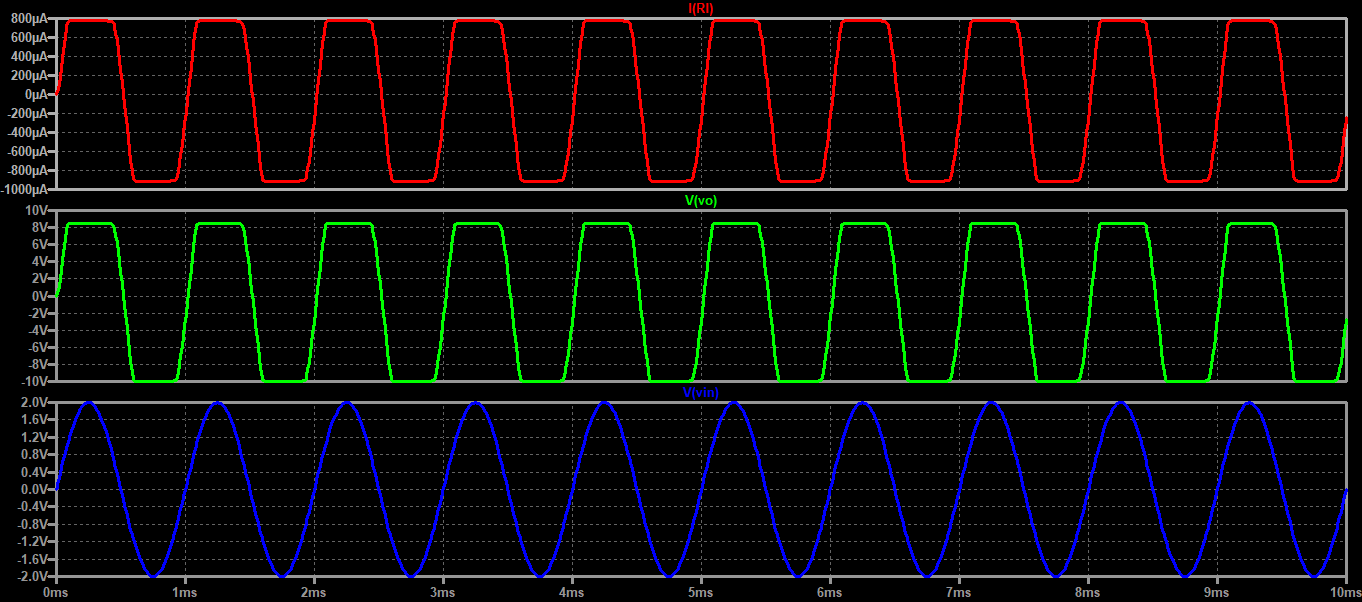
\includegraphics[width=1\textwidth]{figuras/Vout_Vin=2 y R=10k.png}
	\caption{Simulación con $V_{in}=2$[V] y $R_L=10$[K$\Omega$] simulado}
\end{figure}

\subsection{Implementación}


\subsection{Comparación entre resultados}
En la siguiente tabla comparativa se reflejan los resultados obtenidos en cada una de las etapas previas y se calcula el error relativo que existe entre los resultados.\\
Para simplificar los cálculos, se compararon los resultados usando una $R_L=1$[K$\Omega$]
\begin{table}[H]
	\begin{center}
		\begin{tabular}{| c | c | c | c | c |c |c |}
			\hline
			& \multicolumn{3}{ |c| }{Salida $V_o$[V]} &
			\multicolumn{3}{ |c| }{Errores relativos (\%)} \\ \hline
			Entrada $V_{in}$[V] & Teoría & Simulación & Experimental & Exp/Teo & Exp/Sim & Sim/Teo \\ \hline
			0.5  & 0.55 & 0.545	& - & - & - & 0.90 \\
			1    & 1.1  & 1.093	& - & - & - & 0.63 \\
			2    & 2.2  & 2.193	& - & - & - & 0.31 \\ \hline
		\end{tabular}
	\end{center}
\end{table} 

\subsection{Conclusión}
Se puede concluir que la herramienta de simulación es bastante precisa, pues el error relativo respecto al valor teórico siempre se mantuvo menor al 1\%.\\
Ahora bien, el error relativo entre el valor teórico y el experimental es mas grande, aproximadamente (...\%), esto se debe a que los componentes no son ideales y el comportamiento puede variar en un rango acotado indicado por el fabricante.  

 